\documentclass{beamer}

\usetheme{anthem}
\usepackage{lmodern}
%\usepackage{inconsolata}
%\usepackage[scale=.9]{FiraSans}

\title{The \emph{anthem} presentation theme}
\author{Andreas Hinterreiter}
\date{\today}
\titlegraphic{
\includegraphics[height=1cm]{logo}}

\begin{document}

\begin{frame}[plain]
	\titlepage
\end{frame}

\section{A Section with a Figure}

\begin{frame}[plain]
\sectionfigure{
\includegraphics[width=.75\textwidth]{section}}
\sectionpage
\end{frame}

\begin{frame}{An ordinary frame}
\begin{columns}
\column{.5\textwidth}
	\begin{itemize}
		\item An item inside an \texttt{itemize} environment.
		\item Another item.
		\begin{itemize}
			\item A Subitem.
			\item Another, slightly longer subitem.
		\end{itemize}
		\item And, at last, a final item.
	\end{itemize}
\column{.5\textwidth}
	\begin{fancyblock}{A fancy block}
	\raggedright This is the \texttt{fancyblock} environment provided by \emph{anthem}.  It can be customized with \emph{mdframed} options (as seen below).
	\end{fancyblock}
\end{columns}
\end{frame}

\specialsection{A special section}

\begin{frame}[plain]
\sectionfigure{
\includegraphics[width=.75\textwidth]{section}}
\specialsectionpage{Intermezzo}
\end{frame}

\begin{frame}[fragile]{About the Special Sections}
\begin{itemize}
	\item You can declare an \alert{unnumbered special section} using the \verb+\specialsection+ command. This produces a PDF bookmark just like a normal section does.
	\item These special sections have special section title pages created by the \verb+\specialsectionpage{type}+, where the "Part ..." is replaced by \texttt{type}.
	\item Usually, \texttt{type} will be something like "Intermezzo" or "Aside".
\end{itemize}
\end{frame}


\section{An Ordinary Section}

\begin{frame}[plain]
\sectionpage
\end{frame}

\begin{frame}{Another frame}
\begin{columns}
\column{.6\textwidth}
	\begin{enumerate}
		\item An item inside an \texttt{enumerate} environment.
		\item Another item.
		\begin{enumerate}
			\item A Subitem.
			\item Another, slightly longer subitem.
		\end{enumerate}
		\item And, at last, a final item.
	\end{enumerate}
\column{.4\textwidth}
	\begin{fancyblock}[
	innertopmargin=0pt,
	innerbottommargin=0pt,
	innerleftmargin=0pt,
	innerrightmargin=0pt]{A fancy figure}
		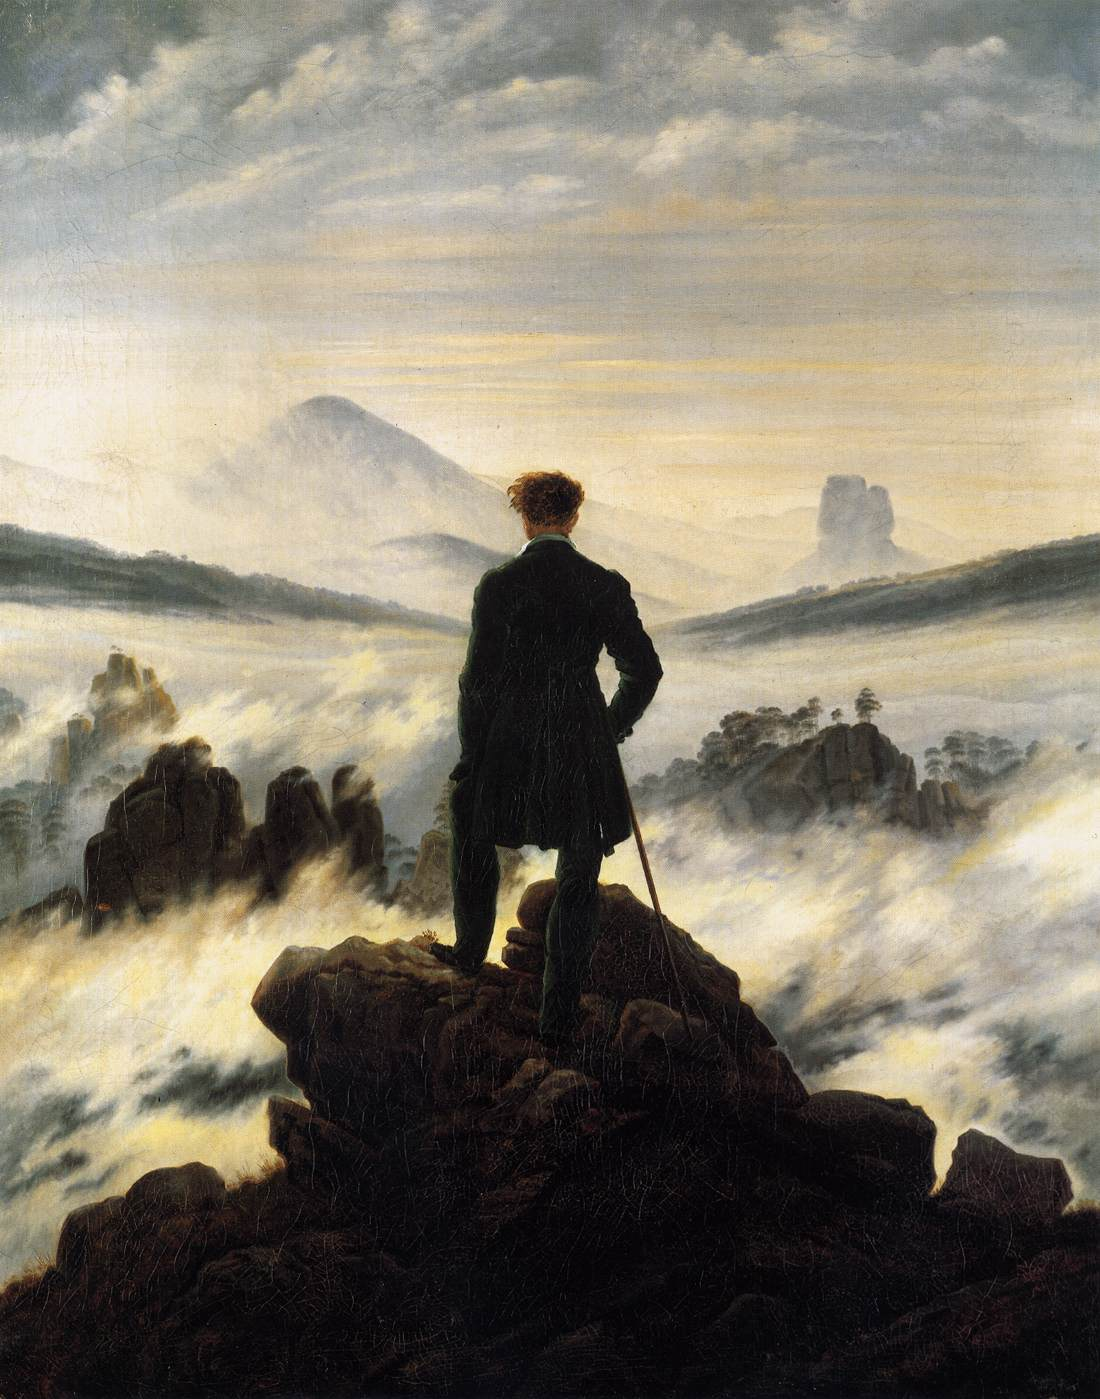
\includegraphics[width=\textwidth]{wanderer}
	\end{fancyblock}
\end{columns}
\end{frame}





\end{document}